
% xetex expected
\documentclass[xetex,professionalfont]{beamer}

% we want math
\usepackage{amsmath}

% fixes and extensions to amsmath
\usepackage{mathtools}

% additional math symbols
\usepackage{amssymb}

% good-looking fractions in text via \sfrac
\usepackage{xfrac}

% fix spaces after custom commands (see below for examples)
\usepackage{xspace}

% minted allows for fancy syntax highlighting (requires python with pygments)
% usage:
%   \begin{minted}{python}
%   codeb
%   \end{minted}
% \usepackage{minted}

% better looking tables
% usage:
%   begin with a \toprule, write a single row of column headings,
%   then add \midrule and after the columns of data we finish with \bottomrule
% example:
%   \begin{tabular}{llr} \toprule
%   Animal & Description & Price \midrule
%   cat & foo & 10 \\
%   dog & bar & 20 \\ \bottomrule
%   \end{tabular}
% note that good tables generally neither have vertical rules nor double rules
\usepackage{booktabs}

% system font support (requires xetex or luatex)
\usepackage{fontspec}
\setmonofont[Scale=0.7]{Cousine} % part of ttf-chromeos fonts on Arch

% improve microtypography
\usepackage{microtype}

% multi-language quotes for babel
\usepackage{csquotes}

% easy way to include copyright information
\usepackage{copyrightbox}

% better bibliographies
\usepackage[backend=biber,style=authoryear]{biblatex}

% language support (english,ngerman)
\usepackage[english]{babel}

% plots (part of texlive-pictures)
\usepackage{pgfplots}

% -----------------------------------------------------------------------------

% specify PDF metadata
\hypersetup{pdftitle={CVSP VO - 3D Vision Applications},pdfsubject={},pdfauthor={Christopher Pramerdorfer}}

% copyright font style
\makeatletter\renewcommand{\CRB@setcopyrightfont}{\tiny\color{lightgray}}

% make emph bold
\DeclareTextFontCommand{\emph}{\bfseries}

% use tuwcvl beamer theme
\usetheme{tuwcvl}

% add bib file
\addbibresource{literature.bib}

% plot setup

\pgfplotsset{width=6.5cm,compat=1.11}

\definecolor{darkgreen}{rgb}{0,0.8,0.1}

% -----------------------------------------------------------------------------

% common english abbreviations
\newcommand{\ie}{\mbox{i.e.}\xspace} % i.e.
\newcommand{\eg}{\mbox{e.g.}\xspace} % e.g.
\newcommand{\wrt}{\mbox{wrt.}\xspace} % wrt.

% math - argmin and argmax
\DeclareMathOperator*{\argmin}{arg\,min}
\DeclareMathOperator*{\argmax}{arg\,max}

\DeclareMathOperator*{\Norm}{Norm}
\DeclareMathOperator*{\Uniform}{Uniform}
\DeclareMathOperator*{\Bern}{Bern}

% shortcuts for number ranges
\newcommand{\NN}{\mathbb{N}}
\newcommand{\ZZ}{\mathbb{Z}}
\newcommand{\QQ}{\mathbb{Q}}
\newcommand{\RR}{\mathbb{R}}

% bold vectors
\renewcommand{\vec}[1]{\ensuremath{\mathbf{#1}}}

% vector shortcuts
\newcommand{\va}{\vec{a}}
\newcommand{\vb}{\vec{b}}
\newcommand{\vc}{\vec{c}}
\newcommand{\ve}{\vec{e}}
\newcommand{\vr}{\vec{r}}
\newcommand{\vs}{\vec{s}}
\newcommand{\vt}{\vec{t}}
\newcommand{\vu}{\vec{u}}
\newcommand{\vv}{\vec{v}}
\newcommand{\vw}{\vec{w}}
\newcommand{\vx}{\vec{x}}
\newcommand{\vy}{\vec{y}}
\newcommand{\vz}{\vec{z}}
\newcommand{\vp}{\vec{p}}
\newcommand{\vq}{\vec{q}}

% bold greek symbols
\newcommand{\bth}{\boldsymbol{\theta}}
\newcommand{\intr}{\boldsymbol{\Lambda}}
\newcommand{\trans}{\mathcal{T}}

% -----------------------------------------------------------------------------

\title{Computer Vision Systems Programming VO}
\subtitle{3D Vision Applications}
\author{Christopher Pramerdorfer}
\institute{Computer Vision Lab, Vienna University of Technology}

\begin{document}

% -----------------------------------------------------------------------------

\begin{frame}
\maketitle
\end{frame}

% -----------------------------------------------------------------------------

\begin{frame}
\frametitle{Topics}

CV applications utilizing scene geometry (3D data)
\begin{itemize}
	\item Focus on those based on Kinect % because it is so popular
\end{itemize}

\bigskip
\begin{center}
    \copyrightbox[b]
    {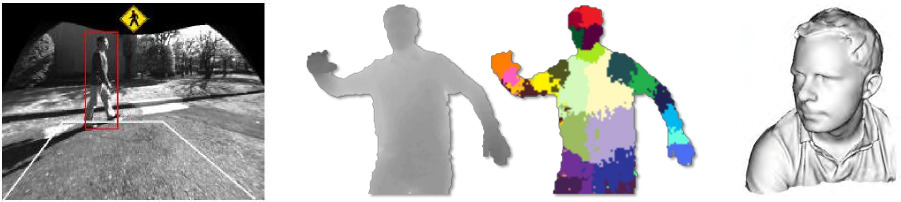
\includegraphics[width=10cm]{figures/intro-collage.jpg}}
    {\centering Images by Ryuzo Okada, \cite{shotton2011}, \cite{newcombe2011}}
\end{center}

\end{frame}

% -----------------------------------------------------------------------------

\begin{frame}
\frametitle{3D Reconstruction}

\begin{center}
    \copyrightbox[b]
    {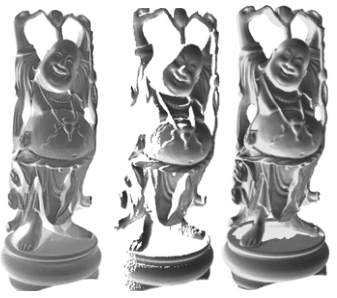
\includegraphics[width=6cm]{figures/3d-reco-tsdf.png}} % photo of the original statue, model from single range scan, model from combined range scans
    {\centering Images from \cite{curless1996}}
\end{center}

\end{frame}

% -----------------------------------------------------------------------------

\begin{frame}
\frametitle{3D Reconstruction}

The obvious thing we can do is generate 3D models
\begin{itemize}
	\item Usually involves combing multiple point clouds % because there are holes due to occlusions / data from point clouds / depth maps / disparity maps ... these are treated as equal because we can map between them ... se previous slide set
\end{itemize}

\bigskip
Accomplished in two steps % these can be alternating, e.g. with kinect fusion
\begin{itemize}
	\item Align range data
	\item Merge range data in a way that minimizes errors % otherwise we could just concatenate the points
\end{itemize}

\end{frame}

% -----------------------------------------------------------------------------

\begin{frame}
\frametitle{3D Reconstruction}
\framesubtitle{Range Data Alignment -- Iterative Closest Points}

Popular method for aligning two point clouds $\{\vr\}$, $\{\vs\}$
\begin{itemize}
	\item Goal is to find parameters $\boldsymbol{\psi}$ of some transformation $\trans$
	\item Usually assuming a rigid transformation % thats a translation + rotation
\end{itemize}

\bigskip
\begin{center}
    \copyrightbox[b]
    {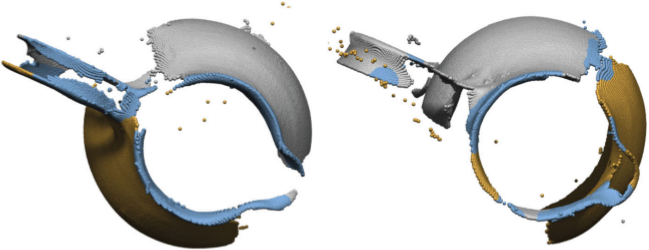
\includegraphics[width=6.5cm]{figures/pot-clouds.png}} % the images are from a different paper, but including them here because they look good
    {\centering Images from \cite{aiger2008}}
\end{center}

\end{frame}

% -----------------------------------------------------------------------------

\begin{frame}
\frametitle{3D Reconstruction}
\framesubtitle{Range Data Alignment -- Iterative Closest Points}

Algorithm iterates between
\begin{itemize}
	\item Finding point correspondences based on distance, $\{(r_n,s_n)\}_n$ % s_i corresponds to r_j if no their distance is below t and if no other s is closer to r_j
	\item Finding the $\boldsymbol{\psi}$ that minimizes $\sum_n\lVert\vr_{r_n}-\trans(\vs_{s_n};\boldsymbol{\psi}) \rVert_2^2$ % this denotes the squares l2 norm ... least squares problem, as the solution to the ML estimate assuming constant additive Gaussian noise ... the minimum can be found in closed form if T is linear (like with a rigid transformation) ... but we still need an iterative approach because the correspondences are erroneous
\end{itemize}

\bigskip
Converges towards a local minimum
\begin{itemize}
	\item Requires good initial estimate of $\boldsymbol{\psi}$
\end{itemize}

\bigskip
\begin{center}
	\url{https://www.youtube.com/watch?v=ii2vHBwlmo8}
\end{center}

% note that ICP always operates on two point clouds. what if we want to align more than two? simply chaining ICP quickly produces bad results because it accumulates errors. but there are some alternatives around ...

\end{frame}

% -----------------------------------------------------------------------------

\begin{frame}
\frametitle{3D Reconstruction}
\framesubtitle{Range Data Merging -- TSDF Fusion}

Truncated signed distance functions (TSDFs)
\begin{itemize}
	\item Similar to distance transforms in 3D (0 = surface)
	\item But distances are signed, measured along view rays 
\end{itemize}

\begin{center}
    \copyrightbox[b]
    {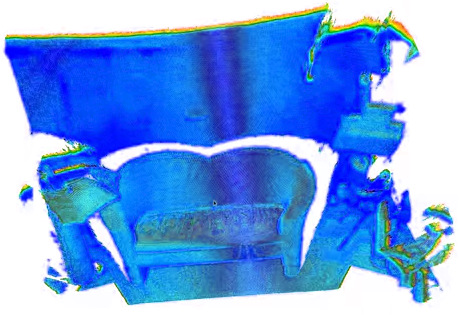
\includegraphics[width=5cm]{figures/tsdf.jpg}}
    {\centering Image from \url{https://www.youtube.com/watch?v=AjjSZufyprU}}
\end{center}

\end{frame}

% -----------------------------------------------------------------------------

\begin{frame}
\frametitle{3D Reconstruction}
\framesubtitle{Range Data Merging -- TSDF Fusion}

Merged data = weighted average over aligned TSDF voxels
\begin{itemize}
	\item Weights based on \eg object distance, angle
\end{itemize}

\begin{center}
    \copyrightbox[b]
    {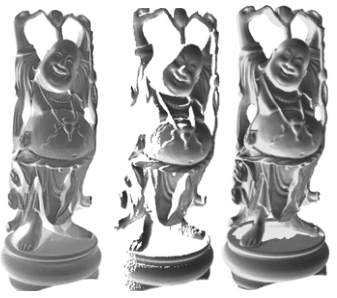
\includegraphics[width=5cm]{figures/3d-reco-tsdf.png}} % photo of the original statue, model from single range scan, model from combined range scans
    {\centering Images from \cite{curless1996}}
\end{center}

\end{frame}

% -----------------------------------------------------------------------------

\begin{frame}
\frametitle{3D Reconstruction}
\framesubtitle{Kinect Fusion}

Temporal fusion of Kinect depth maps

\bigskip
Based on the above methods (ICP \& TSDF fusion)
\begin{itemize}
	\item But $\{\vr\}$ synthesized from merged model
	\item Suppresses alignment error accumulation
\end{itemize}

\begin{center}
    \copyrightbox[b]
    {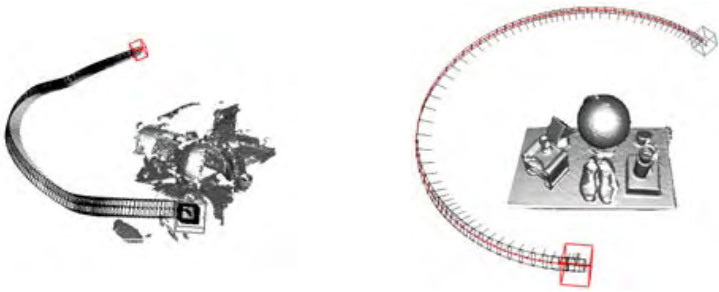
\includegraphics[width=6cm]{figures/kinect-fusion-tracking.jpg}}
    {\centering Images from \cite{newcombe2011}}
\end{center}

\end{frame}

% -----------------------------------------------------------------------------

\begin{frame}
\frametitle{3D Reconstruction}
\framesubtitle{Kinect Fusion}

\begin{center}
	\url{https://www.youtube.com/watch?v=quGhaggn3cQ}
\end{center}

\begin{center}
    \copyrightbox[b]
    {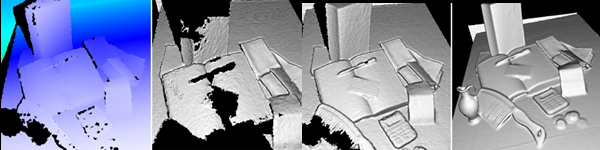
\includegraphics[width=10cm]{figures/kinect-fusion.png}}
    {\centering Images from \url{microsoft.com}}
\end{center}

\end{frame}

% -----------------------------------------------------------------------------

\begin{frame}
\frametitle{3D Reconstruction}
\framesubtitle{Application Fields}

Cultural heritage\\\medskip
Virtual and augmented reality\\\medskip
Architecture\\\medskip
...

\end{frame}

% -----------------------------------------------------------------------------

\begin{frame}
\frametitle{3D Reconstruction}
\framesubtitle{Application Fields}

\begin{center}
	[Video] % show cargo video
\end{center}

\end{frame}

% -----------------------------------------------------------------------------

\begin{frame}
\frametitle{Object Detection}

3D data enables reliable object detection
\begin{itemize}
	\item Metric information available
	\item Invariant to camera parameters % only intrinsics if we don't know the extrinsic parameters though, but we can often auto calibrate to get a sufficient estimate of the extrinsics (as shown below)
\end{itemize}

\end{frame}

% -----------------------------------------------------------------------------

\begin{frame}
\frametitle{Object Detection}
\framesubtitle{Breaking Assistance via Person Detection}

\begin{center}
	\url{https://www.youtube.com/watch?v=oU4XQvxO10k} % the Mercedes also uses radar for this, probably during nighttime? it's also just one example, must manufacturers now have some form of this in their premium models
\end{center}

\begin{center}
    \copyrightbox[b]
    {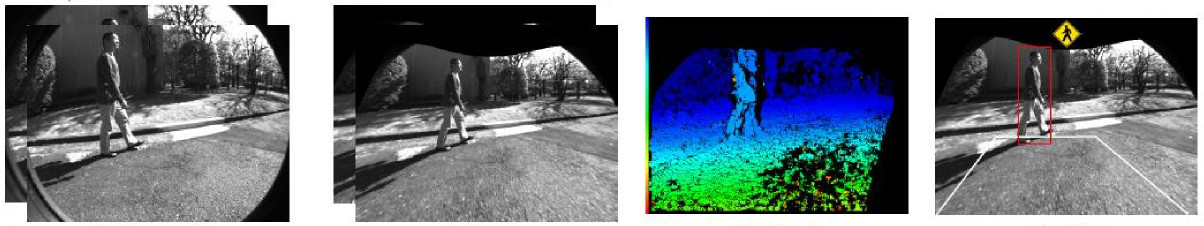
\includegraphics[width=10cm]{figures/car-pedestrian.jpg}}
    {\centering Image from Ryuzo Okada, Toyota}
\end{center}

\end{frame}

% -----------------------------------------------------------------------------

\begin{frame}
\frametitle{Object Detection}
\framesubtitle{Interactive Art Installations}

\begin{center}
    \copyrightbox[b]
    {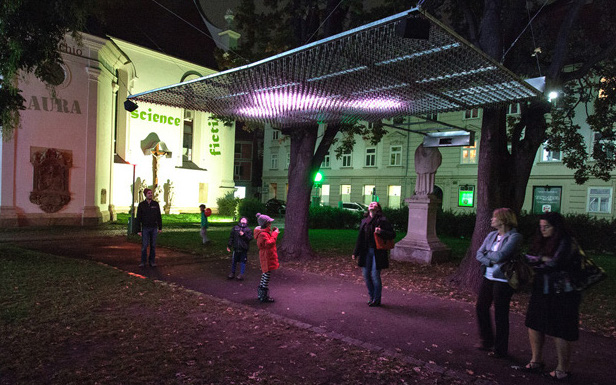
\includegraphics[width=8cm]{figures/ortlos-public-space.jpg}}
    {\centering Image from \url{ortlos.com}}
\end{center}

\end{frame}

% -----------------------------------------------------------------------------

\begin{frame}
\frametitle{Object Detection}
\framesubtitle{Fall Detection (fearless)}

Fall detection system developed at CVL
\begin{itemize}
	\item Uses data from a single Kinect sensor
	\item Runs on an inexpensive single-board computer
\end{itemize}

\bigskip
\begin{center}
    \copyrightbox[b]
    {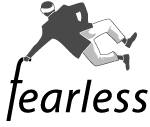
\includegraphics[width=3cm]{figures/fearless.png}}
    {\centering Image from \url{fearless-project.eu}}
\end{center}

\end{frame}

% -----------------------------------------------------------------------------

\begin{frame}
\frametitle{Object Detection}
\framesubtitle{Fall Detection (fearless)}

\begin{center}
	[Video]
\end{center}

\end{frame}

% -----------------------------------------------------------------------------

\begin{frame}
\frametitle{Object Detection}
\framesubtitle{Fall Detection (fearless) -- Motion Detection}

Motion detection via background subtraction
\begin{itemize}
	\item Robust because not affected by illumination, clothing
\end{itemize}

% \bigskip
% Moving parts projected to point cloud in world coordinates
% \begin{itemize}
% 	\item Extrinsics $\boldsymbol{\Omega}$, $\boldsymbol{\tau}$ estimated % see below
% \end{itemize}

\bigskip
\begin{center}
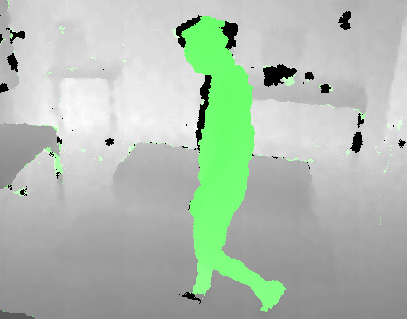
\includegraphics[width=5cm]{figures/fearless-depth.png}
\end{center}

\end{frame}

% -----------------------------------------------------------------------------

\begin{frame}
\frametitle{Object Detection}
\framesubtitle{Fall Detection (fearless) -- Person Detection}

Moving areas projected to point cloud in world coordinates\\\medskip
Person classification based on geometry % on a per-region basis using features like like height, occupied area, volume ... details are not important, this is just an example of how 3D person detection can be accomplished

\bigskip
\begin{center}
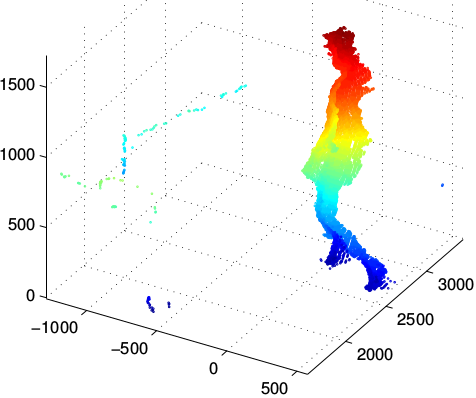
\includegraphics[width=5cm]{figures/fearless-pc.png}
\end{center}

\end{frame}

% -----------------------------------------------------------------------------

\begin{frame}
\frametitle{Object Detection}
\framesubtitle{Fall Detection (fearless) -- Person Detection}

Fall detection based on temporal height change\\\medskip
Furniture detection to reduce false alarm rate

\bigskip
\begin{center}
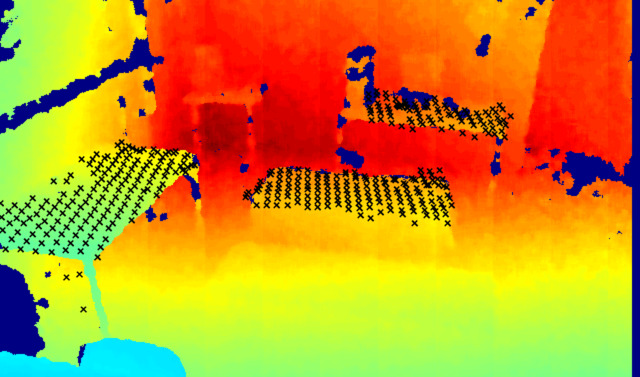
\includegraphics[width=6.5cm]{figures/reclaim-furniture-detection.jpg}
\end{center}

\end{frame}

% -----------------------------------------------------------------------------

\begin{frame}
\frametitle{To Be Continued}

\begin{center}
	More next time!
\end{center}

\end{frame}

% -----------------------------------------------------------------------------

\begin{frame}
\frametitle{Bibliography}

\printbibliography

\end{frame}

\end{document}
